\section{SPI communication}
\label{sec:SPIcommunication}
This section will explain how the connection between the FPGA and the microcontroller is made via an SPI communication protocol. This section can be divided into two parts with the first part concerning the general SPI communication and the second part concerning addressing of the data sendt. Note that the second part has, in principle, nothing to do with the actual SPI communication, however since it is important for both the FPGA microcontroller it makes sense to talk about it bore going into detail with the FPGA and microcontroller.

\subsection{SPI communication protocol}

The SPI communication protocol is used to send data, one bit at a time. The SPI communication protocol runs a master slave relationship which means that one of the parts involved is the master part and fully controls the connection and the other parts simply does what the master part tells them to do. An example of this can be seen on figure \ref{fig:MasterSlave_1_1}.

\begin{figure}[h!]
\centering
\includegraphics[scale=0.5]{Billeder/FPGA/MasterSlave_1_1.png}
\caption{ Diagram of how the master and slave is connected  }
\label{fig:MasterSlave_1_1}
\end{figure}

In order to send the data four wires, called Slave Select (SS), Master out Slave in (MOSI), Master in Slave out (MISO) and Serial Clock (S\_CLK), are used. The MISO and MOSI wires is where the data bits are through and SS and S\_CLK are wires that controls the transfer, note that SS and S\_CLK is controlled only by the master. When the SS is active a data transfer is initiated between the master and a slave, the master is basically saying to the slave that they are now communicating. When the SS is deactivated the transfer is over and all of the data is send. Note that the SS is active low which means that it is active when the SS signal is low and deactivated when the signal is high.  

\newpage

The S\_CLK is used to signal a read of the MOSI and MISO line. This is very important since this is where the synchronization of the data transfer is made. Without this synchronization the data transfer would be impossible.
An example of a SPI data transfer can be seen on figure \ref{fig:SPI_data_transfer}.

\begin{figure}[h!]
\centering
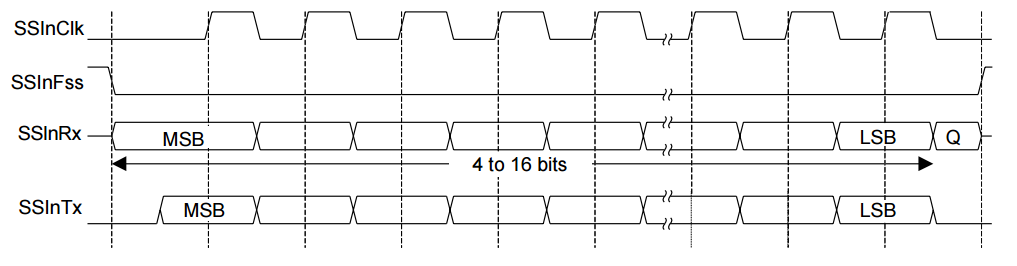
\includegraphics[scale=0.5]{Billeder/FPGA/SPI_data_transfer.png}
\caption{ Illustration of how the package is constructed }
\label{fig:SPI_data_transfer}
\end{figure}

\subsection{Addressing}

Instead of running several SPI slaves in the communication to send the data to the right part of the FPGA, giving the data an address instead was chosen. This makes the amount of data sent longer, however since the controller is a part of the FPGA the speed which information is send does not matter. So since the addressing was found to be the easier solution to make it was chosen.
Addressing works by appending extra bits onto the data, much like a header. An example of this can be seen on figure \ref{fig:Package_Se_1_2}. The address bits then define what kind of data is being send and/or where it has to go. In the case of the SPI slave in the FPGA, the address symbolizes where the data has to go, since what the data symbolizes is an information not needed in the FPGA. In the case of the SPI master in the microcontroller, the address symbolizes what kind of data was received.

\begin{figure}[h!]
\centering
\includegraphics[scale=0.5]{Billeder/FPGA/Package_Se_1_2.png}
\caption{ Illustration of how the package is constructed }
\label{fig:Package_Se_1_2}
\end{figure}

When receiving a packet via the SPI communication, the receiver separates the address from the data and then uses the data according to what the address tells about the data. An example of this can be seen on figure %\# Package\_Re_1_3 \#.

\begin{figure}[h!]
\centering
\includegraphics[scale=0.5]{Billeder/FPGA/Package_Re_1_3.png}
\caption{ Illustration of how the package is destructed }
\label{fig:Package_Re_1_3}
\end{figure}

\newpage











